\documentclass{VUMIFPSkursinis}
\usepackage{algorithmicx}
\usepackage{algorithm}
\usepackage{algpseudocode}
\usepackage{amsfonts}
\usepackage{amsmath}
\usepackage{bm}
\usepackage{caption}
\usepackage{color}
\usepackage{float}
\usepackage{graphicx}
\usepackage{listings}
\usepackage{float}
\usepackage{subfig}
\usepackage{wrapfig}
\usepackage[hidelinks]{hyperref}
\usepackage{todonotes}
\usepackage{xcolor}

% Titulinio aprašas
\university{Vilniaus universitetas}
\faculty{Matematikos ir informatikos fakultetas}
\department{}
\papertype{Programų kūrimo proceso laboratorinis darbas}
\title{Įmonės ,,Mėnuliukų technologijos" programų kūrimo proceso brandos vertinimas}
\titleineng{Maturity assessment of the development process of the ,,Moon Technologies" company}
\status{4 kurso 3 grupės studentai}
\author{Matas Savickis, Justas Tvarijonas, Džiugas Mažulis}
\secondauthor{Greta Pyrantaitė, Andrius Bentkus}

\supervisor{Saulius Ragaišis, Doc., Dr.}
\date{Vilnius – \the\year}

% Nustatymai
% \setmainfont{Palemonas}   % Pakeisti teksto šriftą į Palemonas (turi būti įdiegtas sistemoje)
\bibliography{bibliografija}

\begin{document}
\maketitle

\tableofcontents

\sectionnonum{Įvadas}
	Šiame dokumente aprašysime dabartinio ,,Mėnuliukų technologijos" įmonės programų kūrimo proceso pagerinimą. 
	Prieš procesų gerinimą du procesai iš dalies pasiekia pirmą lygį.
	Šiuo darbu sieksime, kad po proceso pagerinimo trys procesai pasiektų pilną pirmą PKP brandos lygį.

\sectionnonum{Vertinimo apimtis}
	\begin{itemize}
		\item Vertinimo apimtis - visa pirmame darbe aprašyta organizacija.
		\item Aukščiausias vertinamas gebėjimo lygis - maksimalus, kurį procesas gali pasiekti.
		\item Vertinimi procesai:
			\begin{enumerate}
				\item{ENG.1 Reikalavimų išsiaiškinimas}
				\item{ENG.4 Reikalavimų programinei įrangai analizė}
				\item{ENG.5 Programinės įrangos projektavimas}
				\item{ENG.6 Programinės įrangos konstravimas}
				\item{ENG.7 Programinės įrangos integravimas}
				\item{ENG.8 Programinės įrangos testavimas}
				\item{ENG.11 Programinės įrangos instaliavimas}
				\item{ENG.12 Programinės įrangos priežiūra}
				\item{SUP.8 Konfigūracijos valdymas}
				\item{SUP.9 Problemų sprendimas}
				\item{SUP.1 Kokybės užtikrinimas}
				\item{MAN.3 Projekto valdymas}
			\end{enumerate}
	\end{itemize}	

\sectionnonum{Vertinimo rezultatai prieš pagerinimą}
	\begin{figure}[!htbp]
		\includegraphics[scale=1]{img/lentelePries}
		\caption{PKP brandros vertinimo rezultatų lentelė prieš pagerinimą} % Antraštė įterpiama po paveikslėlio
		\label{img:LentelePries}
	\end{figure}

	\begin{figure}[!htbp]
		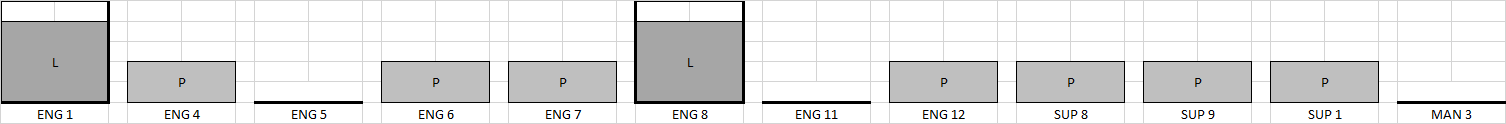
\includegraphics[scale=0.45]{img/ProfilisPries}
		\caption{PKP brandros vertinimo rezultatų gebėjimo profilis prieš pagerinimą} % Antraštė įterpiama po paveikslėlio
		\label{img:ProfilisPries}
	\end{figure}

	\begin{figure}[!htbp]
		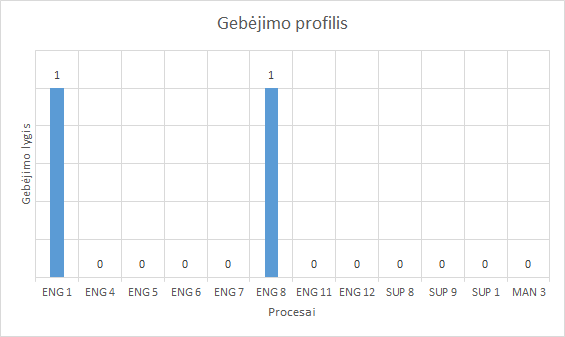
\includegraphics[scale=1]{img/DiagramaProfilisPries}
		\caption{PKP brandros vertinimo rezultatų gebėjimo profilis greinimui prieš pagerinimą} % Antraštė įterpiama po paveikslėlio
		\label{img:DiagramaProfilisPries}
	\end{figure}

\section{Reikalavimų išsiaiškinimo (ENG 1) proceso pagerinimas}

	Buvo nuspręsta padidinti gebėjimo lygį reikalavimo išsiaiškinimo procesui, kadangi šitas procesas kompanijoje atrodo labiausiai išvystitas.
	Taip pat gebėjimas bendrauti su užsakovais ir tiksliai išsiaiškinti reikalavimus atrodo kaip labai reikalingas pradinis žingsnis kiekvienoje įmonėje.
	Visi kiti procesai gali būti tobuli, tačiau jeigu pradiniai reikalavimai būs netinkamai arba blogai užrašyti ir išsiaikinti, like procesai būs gamins tiesiog netinkamą produktą.

\subsection{Pagerinimas}

	\begin{enumerate}
		\item{Išreikštinai pridedamas bendravimas su būsimos programų sistemos vartotojais reikalavimų cikle.}
		\item{Išreikštinai surenkami parašai is galutinių vartotojų, užsakovų ir tiekėjų, kad reikalavimai buvo suprasti, kaip užrašti jie dokumente.}
		\item{Aiškiau aprašomas defekto analizės procesas.}
		\item{Pridėtas reikalavimų stebėjimo mechanizmas naudojant programinę sistemą, ne vien naudojamasi dokumentais.}
	\end{enumerate}
	\subsubsection{Proceso aprašymas po pagerinimo}
	\begin{center}
		\begin{table}[ht]
			\caption{Reikalavimų ciklo procesas.}
			\begin{tabular}{ | l | l | }
				\hline
				Pavadinimas:		& Reikalavimų ciklas.												\\ \hline
				Tikslas:		& Suformuoti funkcinius ir nefunkcinius reikalavimus.								\\ \hline
				Vykdytojai:		& Programuotojas, analistas, klientas.										\\ \hline
				Veiklos:		& V1 - Iš kliento pateiktų verslo reikalavimų suformuojame funkcinius \\ & reikalavimus. 			\\
	
							& V2 - Pristatome klientui sudarytus funkcinius reikalavimus ir tiksliname \\& pateiktus verslo reikalavimus.	\\
							& V3 - Siūlomi nefunkciniai reikalavimai.									\\ \hline
				Naudojami produktai:	& NP1 - Kliento pateiktas verslo reikalavimų dokumentas.							\\ \hline
				Sukuriami produktai:	& SP1 - Funkcinių ir nefunkcinių reikalavimų dokumentas.							\\ \hline
							& SP2 - Susaistytų šalių parašai reikalavimam patvirtinti.							\\ \hline
			\end{tabular}
		\end{table}
	\end{center}
	
	\begin{enumerate}
		\item{
			Iš užsakovo ir naudotojų pateiktų verslo reikalavimų suformuojame funkcinius ir nefunkcinius reikalavimus.
			Su visom partijom, įskaitant užsakovus ir naudotojus, susėdama, aptariami reikalavimai ir taip suderinami, kad visos susaistytos šalys būtų patenkintos.
			Iš visų partijų surenkami parašai, tam kad vėliau nekiltų klausimų, kodėl reikalavimai neatitinka įsivaizdavimų.
			Mūsų įmonės verslo analitikas dirbdamas kartu su programuotojais suformuoja atsekamus (su indentifikacijos kodu) funkcinius ir nefunkcinius reikalavimus.
		}
		\item{
			Kompanija pateikia prieigą prie sistemos, su visu reikalavimų sąrašu, kur užsakovai gali stebėti jų įvykdymą.
			Testuojant suprogramuotą funkcionalumą ir įgyvendinus reikalavimą, sistemoje pažymimas jog reikalavimas įgyvendintas.
		}
		\item{
			Išsiaiškinami baziniai reikalavimai, kurie yra patys svarbiausi ir turi būti pirmi igyvendinti, baziniai reikalavimai yra atitinkamai pažymimi sistemoje.
			Baziniai reikalavimai yra ypač atidžiai analizuojami analistų, analizėje taip pat įvertinama, kokia tikimybė, jog pasikeis reikalavimas ir atitinkamai suplanuojami veiksmai tokiu atveju.
		}
		\item{
			Pristatome klientui sudarytus funkcinius reikalavimus ir tiksliname pateiktus verslo reikalavimus - suformavus funkcinius reikalavimus planuojami susitikimai su klientu, siekiant jam pristatyti suformuotus reikalavimus, patikslinti pateiktus verslo reikalavimus ir toliau tikslinti reikalavimus iki kol reikalavimai tenkins klientą ir bus suprantami programuotojų komandai, kuri dirbs prie kliento projekto.
		}
		\item{
			Siūlomi nefunkciniai reikalavimai - jeigu klientas pats nepateikė nefunkcinių reikalavimų įmonė pati pateikia nefunkcinių reikalavimų siūlymus pagal esamo projekto apimtį ir biudžetą.
			Pateikti nefunkciniai reikalavimai yra aptariami ir tikslinami su klientu.
		}
		\item{
			Jeigu klientas reikalavimą pakeičia programavimo fazėje tai reikalavimas yra atidžiai peržiūrimas dar kartą, įvertinama, kiek kitokio funkcionalumo reikės pakeisti kuriamoj programų sistemoje, ir klientui pateikiama nauja sutartis, kurioje aprašoma, kokie darbai bus atlikti tam, kad jau suprogramuotoje sistemoje pakeistas reikalavimas būtų įgyvendintas.
			Dar neįgyvendintų reikalavimų keitimas yra pigesnis (nes nereikia perprogramuoti nieko) ir klientui aiškiai išdėstoma kainos struktūra, kiek nauja sutartis kainuos, jeigu būs keičiami reikalavimai, kurie jau įgyvendinti.
		}
	\end{enumerate}
	\begin{figure}[h!]
		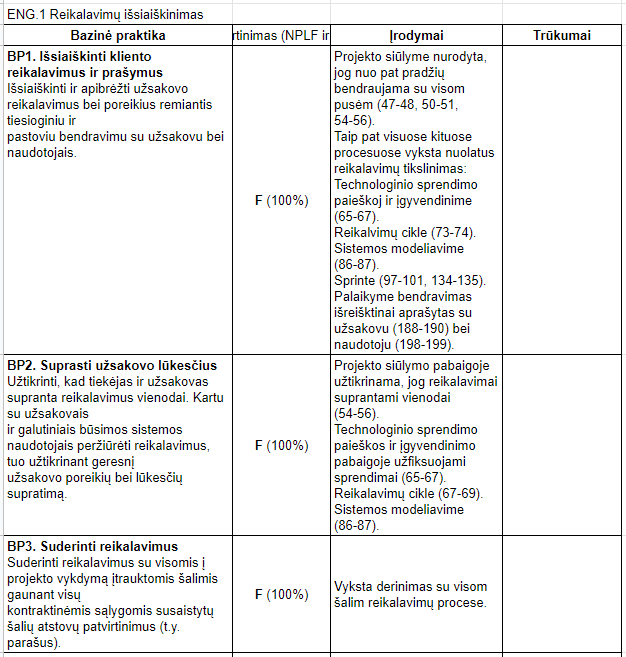
\includegraphics[scale=1]{img/eng1one}
		\caption{PKP ENG1  proceso branda po pagerinimo} % Antraštė įterpiama po paveikslėlio
		\label{img:pkpPries}
	\end{figure}
\newpage
	\begin{figure}[h!]
		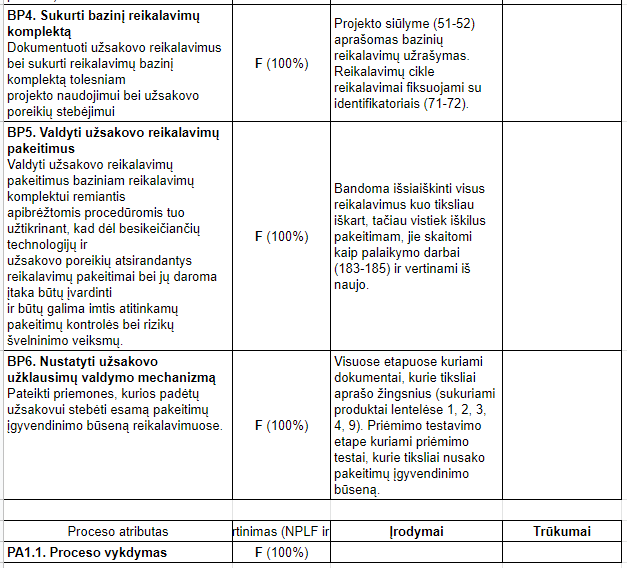
\includegraphics[scale=1]{img/eng1two}
		\caption{KP ENG1 proceso branda po pagerinimo} % Antraštė įterpiama po paveikslėlio
		\label{img:pkpPries}
	\end{figure}
	\newpage

\section{Programinės įrangos testavimo (ENG 8) proceso pagerinimas}	
	Kadangi labai svarbus klientų pasitikėjimas mūsų produkto kokybe, pasirinkome gerinti programinės įrangos testavimo procesą. Testuodami norime užtikrinti, kad perdavus klientui produktą neatsiras kalnas problemų ir jis veiks visose aplinkose, kuriose turi veikti.
	\subsection{Pagerinimas}
	Buvo įvesti keli pagerinimai kokybės užtikrinimo skyriuje:
	\begin{enumerate}
						\item Prie sukuriamų produktų pridedama vartotojo dokumentacija.
						\item Pridėtas pradinių duomenų apibrėžimas.
						\item Paminėta, kad sudaryti testai padengia visus su testuojama užduotim susijusius reikalavimus.
	\end{enumerate}
	Pagrinde, ką reikėjo padaryti, kad pagerinti procesą, tai papildyti ir detaliau aprašyti dokumentaciją - testai tie patys: modulių, integraciniai, automatizuojami, regresiniai testai, bet aiškiau aprašyta, kokio rezultato po testavimo tikimasi.
	\subsubsection{Proceso aprašymas po pagerinimo}
	\begin{center}
		\begin{table}[ht]
			\caption{Kokybės užtikrinimo procesas}
			\begin{tabular}{ | l | l | }
				\hline
				Pavadinimas:		& Kokybės užtikrinimas.							\\ \hline
				Tikslas:		& Pasirūpinti, kad sistema su atnaujinta kodo baze veiktų teisingai.	\\ \hline
				Vykdytojai:		& Testuotojai ir programuotojai.					\\ \hline
				Veiklos:		& V1 - Rašomi modulių testai.						\\
							& V2 - Rašomi integraciniai testai.					\\
							& V3 - Rašomi automatizuojami testai.					\\
							& V4 - Vykdomas regresinis testavimas.					\\
							& V5 - Testų klaidų analizė ir defektų aprašymas.			\\ \hline
				Naudojami produktai:	& NP1 - Užduočių sąrašas. 						\\
							& NP2 - Testai regresiniam testavimui.					\\ \hline
				Sukuriami produktai:	& SP1 - Nauji defektai.							\\
							& SP2 - Testų rezultatų dokumentas.					\\
							& SP3 - Papildytas naujais defektais užduočių sąrašas.			\\ 
							& SP4 - Vartotojo dokumentacija. \\ \hline
			\end{tabular}
		\end{table}
	\end{center}

	Kokybės užtikrinimas skirtingas kiekvienam projektui.
	Tuose projektuose, kuriuose kuriamoje sistemoje egzistuoja vartotojo sąsaja, atliekamas rankinis testavimas kartu su automatizuotu regresiniu testavimu. Kiekvienas testas apibrėžia pradinius duomenis ir tikrina rezultatus. Šie sudaryti testai turi padengti visus užduoties bei programinės įrangos reikalavimus ir užtikrinti, kad rezultatai atitinka užduoties aprašymą bei nesugriauna kitų programos dalių.
	Į kokybės užtikrinimą yra įtraukiami ir programuotojai, kurie yra atsakingi už modulių testų rašymą ir klaidų taisymą.
	Testuotojai atsakingi už rankinį testavimą, automatizuotų testų rašymą bei regresinių testų rezultatų apibendrinimą.
	Jeigu projektas yra iteracinis ir jau išleistas plačiam naudojimui, po sėkmingo testavimo kodas yra sudedamas į aukštesnę aplinką, kurioje yra papildomai pravaliduojamas prieš jį išleidžiant į produkciją.
	Jei testavimas parodė defektus - jie užregistruojami kaip užduotys ir jų taisymui, pagal jų sunkumą, skiriamas prioritetas. 
Atlikus testavimus, jei vartotojo dokumentacija dar neparašyta vartotojo dokumentacija, ji parašoma implementuotom užduotim, o jei jos nėra, ji atnaujinama.
	\par
	Ir programuotojai ir testuotojai atsakingi už tvarkingą ir kokybišką kodą ir sklandų programos veikimą.
	Viena rečiau minima kokybės užtikrinimo dalis yra kodo peržiūra.
	Kiekvienas programuotojas yra atsakingas už kitų savo rato programuotojų kodo peržiūrą (angl. Pull Request review) prieš jo kėlimą į aukštesnes aplinkas.
	Taip išvengiama kartais net labai sunkių klaidų dėl vieno ar kelių žmonių apsižiūrėjimo.
	Tuo pačiu išvengiama nedarbingo laiko, kuris atsirado dėl kitų programos dalių sulaužančio kodo įdėjimo į pagrindinę ''master'' kodo bazę.

	\newpage
	
	\subsection{NPLF atitikimas po pagerinimo}
	\begin{figure}[!htbp]
		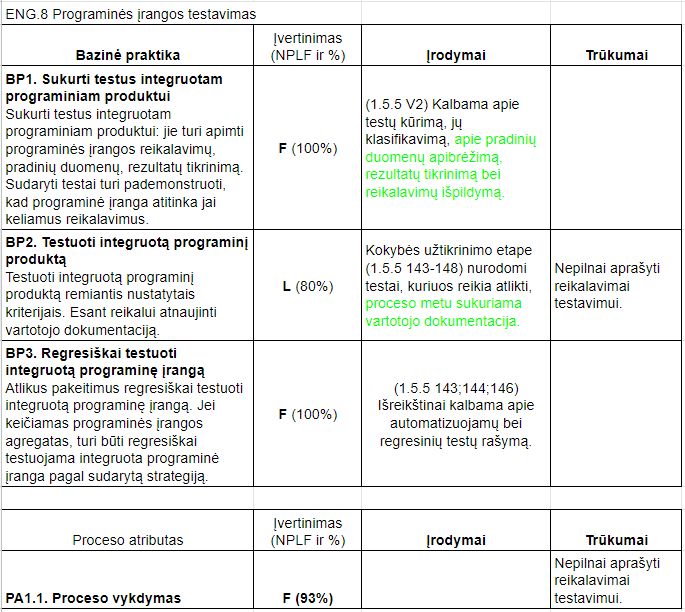
\includegraphics[scale=0.9]{img/eng8_po_pakeitimo}
		\caption{PKP ENG8 proceso branda po pagerinimo} % Antraštė įterpiama po paveikslėlio
		\label{img:pkpPries}
	\end{figure}
	
\section{Kokybės užtikrinimo (SUP 1) proceso pagerinimas}
	Pasirinkome pagerinti kokybės užtikrinimo procesą, nes manome, kad siekiant išlaikyti esamus klientus ir pritraukti ateities klientus svarbiau yra užtikrinti, 
	kad sukurtos programos būtų paprastos ir kokybiškos, negu su daug funkcionalumų, tačiau prastai veikiančios.

			\subsection{Pagerinimas}
				Įvedamos procesų gerinimo metrikos.
				Pradėjus naują projektą kiekvieno proceso metu projektų vadovas žymisi metrikas apie procesą.
					\begin{enumerate}
						\item{Proceso unikalus indikatorius (kiekvienam projektui skirtingas)}
						\item{Kokia buvo numatyta proceso trukmė}
						\item{Kiek laiko truko procesas}
						\item{Ar visos numatytos šalys dalyvavo projekte}
						\item{Kiek proceso veiklų buvo įgyvendinta}
						\item{Proceso kaina}
						\item{Atsiliepimai apie procesą}
					\end{enumerate}
				Pagal šias metrikas projekto pabaigoje, per projekto aptarimą, yra vykdomas pačio proceso aptarimas ir, jeigu to reikia, gerinimas.

				Jeigu projekto vadovas mato, kad pačio projekto vykdymo metu būtinas proceso pakeitimas, yra daromas susirinkimas su kompanijos savininkais ir suinteresuotais asmenimis siekiant spręsti šį klausimą. 
				Jeigu reikia, proceso modelio gerinimo procesas yra pradedamas anksčiau ir modelio pakeitimai yra įgyvendinami kaip galima greičiau.

\pagebreak
	\begin{center}
		\begin{table}[ht]
			\caption{Programų kūrimo proceso gerinimo procesas}
			\begin{tabular}{ | l | l | }
				\hline
				Pavadinimas:		& Proceso gerinimas.						\\ \hline
				Tikslas:		& Aptarti praėjusio projekto programų kūrimo procesą ir pagerinti jį.			\\ \hline
				Vykdytojai:		& Įmonės darbuotojai, dirbę prie projekto, ir įmonės vadovybė.					\\ \hline
				Veiklos:		& V1 - Aptariamas kiekvienas modelio procesas. 				\\
							& V2 - Apžvelgiamos metrikos.	\\
							& V3 - Surašomi gerinimo pasiūlymai.				\\ 
							& V4 - Atliekama proceso gerinimo atsiperkamumo analizė \\ 
							& V5 - Sudaromas naujas programų sistemų kūrimo modelis \\ \hline
				Naudojami produktai:	& NP1 - Proceso gerinimo metrikos. 				\\ \hline
				Sukuriami produktai:	& SP1 - Pagerintas programų kūrimo proceso modelis.		\\ \hline
			\end{tabular}
		\end{table}
	\end{center}

	\begin{enumerate}
		\item{Bendrais bruožais aptariamas kiekvienas modelio procesas, kokia komandos nuomonė, kaip sekėsi sekti proceso nurodymus jų pačių akimis ir ar procesas jiems padėjo.}
		\item{Apžvelgiamos metrikos ir kaip jos atsispindi tame, kas buvo kalbama pirmoje veikloje. 
			Išsiaiškinama, kodėl nebuvo laikomasi proceso nurodymų, kodėl jis užtruko ilgiau arba trumpiau negu planuota, ir kodėl buvo sunaudota daugiau arba mažiau pinigų negu planuota.}
		\item{Kiekvienas susirinkimo dalyvis anonimiškai surašo savo pasiūlymus, kaip gerinti procesą.
			Pasiūlymai peržiūrimi susitikimo dalyvių ir iškeliama diskusija trumpai aptariant visus nesidubliuojančius pasiūlymus.}
		\item{Pagal atrinktus pasiūlymus ir vadovybės išskirtus proceso gerinimo tikslus įvertinama, kiek kiekviena gerinimo veikla kainuos implementuoti į modelį ir koks bus trumpalaikis ir ilgalaikis veikos atsiperkamumas.}
		\item{Atmetus nereikalingus tikslus sukuriamas naujas programų sistemos kūrimos proceso modelis, kuriuo bus vadovaujamasi kituose projektuose.}
	\end{enumerate}

	Pastaba: jeigu modeliui pasikeitus projektas vis dar vyksta ir pakeitimai nėra kritiniai, liekama prie senos modelio versijos siekiant negluminti užsakovo.	

	\begin{figure}[!htbp]
		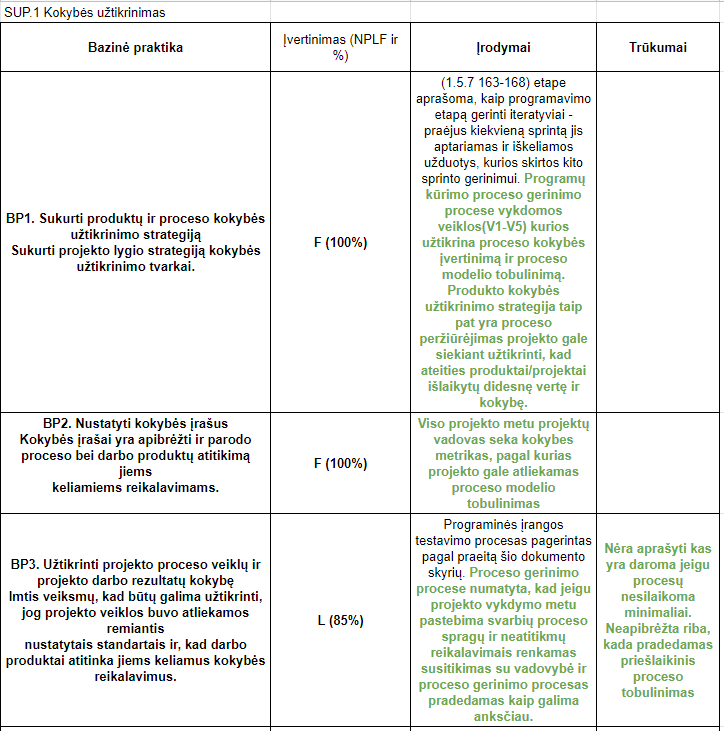
\includegraphics[scale=0.9]{img/sup1one}
		\caption{PKP SUP1 proceso branda po pagerinimo} % Antraštė įterpiama po paveikslėlio
		\label{img:pkpPries}
	\end{figure}	

	\begin{figure}[!htbp]
		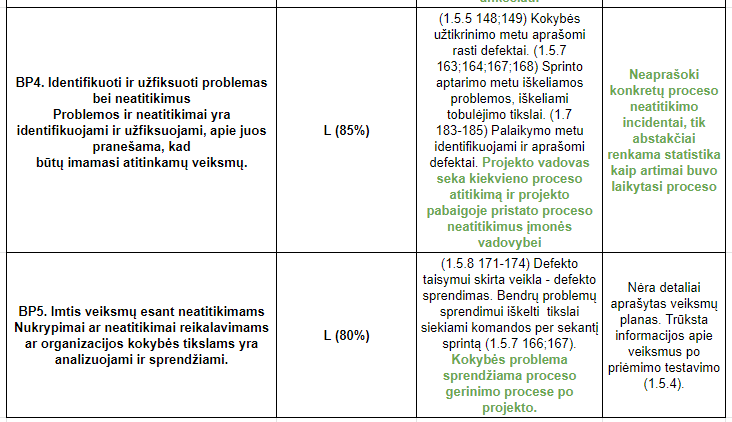
\includegraphics[scale=0.9]{img/sup1two}
		\caption{PKP SUP1 proceso branda po pagerinimo} % Antraštė įterpiama po paveikslėlio
		\label{img:pkpPries}
	\end{figure}	

	\subsection{NPLF atitikimas po pagerinimo}

	\begin{figure}[!htbp]
		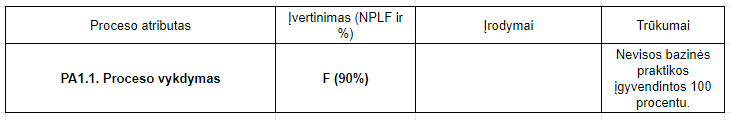
\includegraphics[scale=0.9]{img/sup1three}
		\caption{PKP SUP1 proceso branda po pagerinimo} % Antraštė įterpiama po paveikslėlio
		\label{img:pkpPries}
	\end{figure}	

\sectionnonum{Vertinimo rezultatai po pagerinimo}
	\begin{figure}[!htbp]
		\includegraphics[scale=1]{img/lentelePo}
		\caption{PKP brandros vertinimo rezultatų lentelė po pagerinimo} % Antraštė įterpiama po paveikslėlio
		\label{img:LentelePo}
	\end{figure}

	\begin{figure}[!htbp]
		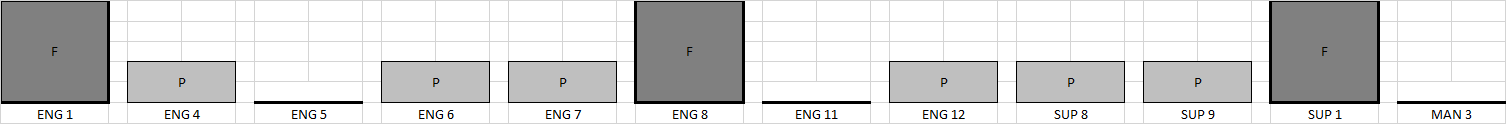
\includegraphics[scale=0.45]{img/ProfilisPo}
		\caption{PKP brandros vertinimo rezultatų gebėjimo profilis po pagerinimo} % Antraštė įterpiama po paveikslėlio
		\label{img:ProfilisPo}
	\end{figure}

	\begin{figure}[!htbp]
		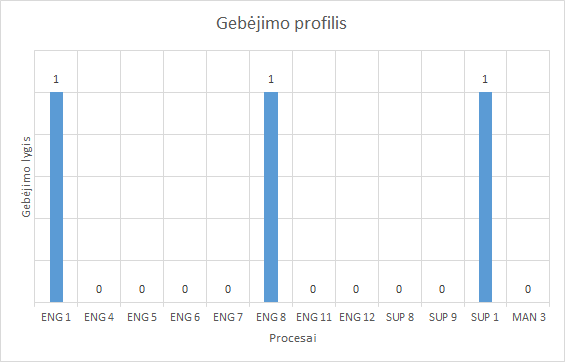
\includegraphics[scale=1]{img/DiagramaProfilisPo}
		\caption{PKP brandros vertinimo rezultatų gebėjimo profilis greinimui po pagerinimo} % Antraštė įterpiama po paveikslėlio
		\label{img:DiagramaProfilisPo}
	\end{figure}

\sectionnonum{Rezultatai ir išvados}
	Po procesų pagerinimo pavyko sėkmingai pakelti tris procesus iki pilno pirmo PKP brandos lygio. 
	Išsiaiškinom ir supratom, kad net ir nedideli bet tikslingi pakeitimai procese padaro daug teigiamos įtakos kokybei. 

\end{document}
